% !TEX root = ../main.tex
\section{鲁棒约束下的第二检测点选择}

\subsection{问题分析与建模思路}

问题二已知某全向干扰源在第一个检测点处的示向度，要求确定第二个检测点的选择策略及候选区域。第二个检测点既要与第一次示向方向形成较大的交会角，以减弱角度误差对定位结果的放大作用，又要尽可能位于干扰源的有效接收范围内。由于不同干扰源的有效接收半径未知，但均属于 $[1000,1500]$ 米，因此第二次检测应优先利用 $1000$ 米的共同下界建立确定性的接收保证。在此基础上，以连续最坏定位损失为理论主目标，以移动时间为次目标，并用有限网格给出可复现的离散近似。

本节沿用问题一的半平面表示。首先根据第一次观测构造干扰源候选区域，然后给出满足接收保证的第二检测点区域，并将其分为第一次示向线左右两侧的两个候选子区域。理论上使用全部已有信息更新二次位置可行域；数值上以圆域外接多边形复用问题一的半平面交和直径算法，得到有限网格下的近似优良检测位置。

\subsection{第一次观测后的干扰源候选区域}

设第一个检测点为 $S_1=(x_1,y_1)$，测得示向度为 $\theta_1$，测向误差上限仍记为 $\varepsilon=\pi/180$。由式~\eqref{eq:q1-wedge}，第一次观测对应的示向角形区域为 $W_1$。记目标圆域为
\begin{equation}
  D=\left\{G:\|G\|_2\leq1800\right\}.
  \label{eq:q2-target-disk}
\end{equation}

由于已经获得示向度，说明第一个检测点位于该干扰源的有效接收范围内。虽然干扰源的真实有效接收半径未知，但其上界为 $1500$ 米，因此真实源位置必定位于 $B(S_1,1500)$ 内。为保持候选区域的凸性并给出保守的接收保证，先暂不利用“距离超过 $5$ 米”这一微小的近距离排除条件，定义扩大的凸候选区域为
\begin{equation}
  C_1=D\cap W_1\cap B(S_1,1500).
  \label{eq:q2-first-region}
\end{equation}
式~\eqref{eq:q2-first-region} 同时包含目标区域约束、第一次示向约束和最大接收距离约束。由于第一次检测得到的是示向度而非“距离过近”提示，物理上与该次观测相容的有效源集还应满足 $\|G-S_1\|_2>5$，记为
\[
  C_1^{\mathrm{dir}}
  =\left\{G\in C_1:\|G-S_1\|_2>5\right\}.
\]
后续构造保证接收区域时仍使用扩大的凸集 $C_1$，以保持接收保证的保守性；涉及真实方位角、交会角和定位损失时则使用 $C_1^{\mathrm{dir}}$，从而避免零向量方向未定义的问题。

需要注意，第一次检测成功只能推出 $\|G-S_1\|_2\leq1500$，不能推出 $\|G-S_1\|_2\leq1000$。这是因为真实有效接收半径可能取 $1000$ 至 $1500$ 米之间的任意值。

\subsection{交会角与定位误差的关系}

设真实干扰源位置为 $G$，第二个检测点为 $q$。从两个检测点指向干扰源的方向向量分别为 $G-S_1$ 和 $G-q$，两次示向线的交会角定义为
\begin{equation}
  \phi(G,q)=\angle(G-S_1,G-q),
  \qquad 0\leq\phi(G,q)\leq\pi.
  \label{eq:q2-cross-angle}
\end{equation}

在小误差线性化条件下，位置误差中包含如下交会几何放大因子：
\begin{equation}
  \kappa(G,q)=\frac{1}{|\sin\phi(G,q)|}
  \label{eq:q2-amplification}
\end{equation}
当 $\phi$ 接近 $0$ 或 $\pi$ 时，两条示向线近乎平行或反平行，$\kappa$ 急剧增大；当 $\phi$ 接近 $\pi/2$ 时，$\kappa$ 取得最小值。实际位置误差还受两次观测距离影响，因此 $\kappa$ 只用于几何解释和搜索引导，候选点的最终评价仍以定位区域直径为准。

但是，若机器狗只在 $S_1$ 处沿垂直于示向线的方向移动，则其与远距离干扰源的距离可能进一步增大，导致第二次检测无法接收到信号。因此，本节采用“沿示向方向前进并向一侧偏移”的候选点结构，在接收可靠性和交会角之间取得平衡。

\subsection{保证接收区域与候选区域}

由于所有全向干扰源的有效接收半径均不小于 $1000$ 米，只要第二检测点到 $C_1$ 内任意可能源位置的距离均不超过 $1000$ 米，即可保证第二次检测收到信号。定义保证接收区域
\begin{equation}
  Q_{\mathrm{det}}
  =\left\{
  q:\max_{G\in C_1}\|q-G\|_2\leq1000
  \right\}
  =\bigcap_{G\in C_1}B(G,1000).
  \label{eq:q2-detection-region}
\end{equation}

下面说明式~\eqref{eq:q2-detection-region} 在本题条件下非空。定义第一次示向中心方向的单位向量
\begin{equation}
  \mathbf u=
  \begin{pmatrix}
    \cos\theta_1\\
    \sin\theta_1
  \end{pmatrix},
  \label{eq:q2-center-direction}
\end{equation}
并在中心示向线上取点
\begin{equation}
  q_0=S_1+750\mathbf u.
  \label{eq:q2-feasible-point}
\end{equation}
任取 $G\in C_1$，均可将其表示为
\begin{equation}
  G=S_1+r
  \begin{pmatrix}
    \cos(\theta_1+\delta)\\
    \sin(\theta_1+\delta)
  \end{pmatrix},
  \qquad 0\leq r\leq1500,\qquad |\delta|\leq\varepsilon.
  \label{eq:q2-source-parameterization}
\end{equation}
这里仅使用 $C_1\subseteq B(S_1,1500)\cap W_1$ 得到的必要范围；目标圆域 $D$ 只会进一步缩小不同方向上 $r$ 的可取区间。因此，在式~\eqref{eq:q2-source-parameterization} 所示扩大参数域上得到的距离上界，对真实集合 $C_1$ 仍是有效的保守上界。
由余弦定理，$q_0$ 与 $G$ 的距离满足
\begin{equation}
  \|q_0-G\|_2^2
  =r^2+750^2-1500r\cos\delta.
  \label{eq:q2-feasible-distance}
\end{equation}
对于固定的 $\delta$，式~\eqref{eq:q2-feasible-distance} 关于 $r$ 为凸二次函数，其在区间 $[0,1500]$ 上的最大值于端点取得。当 $r=0$ 时距离为 $750$ 米；当 $r=1500$ 且 $|\delta|=1^\circ$ 时，距离约为 $750.23$ 米。因此
\begin{equation}
  \max_{G\in C_1}\|q_0-G\|_2<751<1000,
  \label{eq:q2-nonempty-proof}
\end{equation}
从而 $q_0\in Q_{\mathrm{det}}$，保证接收区域必定非空。进一步由三角不等式，对任意满足 $\|q-q_0\|_2<249$ 的点，均有
\[
  \|q-G\|_2
  \leq\|q-q_0\|_2+\|q_0-G\|_2<1000,
  \qquad G\in C_1.
\]
故 $B^\circ(q_0,249)\subseteq Q_{\mathrm{det}}$，这也直接说明 $q_0$ 左右两侧均存在保证接收的候选点。

为描述候选区域的左右结构，定义垂直于 $\mathbf u$ 的单位向量
\begin{equation}
  \mathbf n=
  \begin{pmatrix}
    -\sin\theta_1\\
    \cos\theta_1
  \end{pmatrix}.
  \label{eq:q2-normal-direction}
\end{equation}
任意第二检测点可写为
\begin{equation}
  q=S_1+a\mathbf u+b\mathbf n,
  \label{eq:q2-candidate-parameterization}
\end{equation}
其中 $a$ 表示沿中心示向方向的前进距离，$b$ 表示侧向偏移量。本文采用基于 $1000$ 米统一接收下界的保守可靠候选区域
\begin{equation}
  Q_{\mathrm{cand}}=Q_{\mathrm{det}}.
  \label{eq:q2-candidate-region}
\end{equation}
为描述候选域相对于第一次中心示向线的左右结构，根据 $b$ 的正负定义两个子区域
\begin{align}
  Q_{\mathrm L}
  &=\left\{q\in Q_{\mathrm{cand}}:b>0\right\},
  \label{eq:q2-left-region}\\
  Q_{\mathrm R}
  &=\left\{q\in Q_{\mathrm{cand}}:b<0\right\}.
  \label{eq:q2-right-region}
\end{align}
式~\eqref{eq:q2-left-region} 与式~\eqref{eq:q2-right-region} 分别给出第一次中心示向线左、右两侧的候选子区域。由 $B^\circ(q_0,249)\subseteq Q_{\mathrm{det}}$ 可知，对充分小的 $\eta>0$，点 $q_0\pm\eta\mathbf n$ 仍属于 $Q_{\mathrm{cand}}$，左右两个子区域均非空。中心示向线和其他边界点虽然通常会因交会角较差而被目标函数淘汰，但仍保留在整个保守候选域中，避免在没有全局证明时提前删除潜在可行解。数值程序不预先排除任一侧，而是在由接收约束推导的完整必要包围盒内统一搜索。

\subsection{最坏定位直径模型}

对于候选点 $q$ 和可能的真实源位置 $G\in C_1^{\mathrm{dir}}$，当 $\|q-G\|_2>5$ 时，第二检测点指向干扰源的真实方位角为
\begin{equation}
  \beta(q,G)=\operatorname{atan2}(G_y-q_y,G_x-q_x),
  \qquad \|q-G\|_2>5.
  \label{eq:q2-true-bearing}
\end{equation}
设第二次测量误差为 $e_2\in[-\varepsilon,\varepsilon]$，则第二次实际测得的示向度可表示为
\begin{equation}
  \theta_2=\operatorname{wrap}_{[0,2\pi)}\bigl(\beta(q,G)+e_2\bigr).
  \label{eq:q2-second-bearing}
\end{equation}

由检测点 $q$ 和示向度 $\theta_2$ 构造第二个角形区域 $W_2(q,\theta_2)$。为利用目标圆域、第一次示向和最大接收距离等全部已有信息，第二次观测后的位置可行域定义为
\begin{equation}
  P_2(q,G,e_2)
  =C_1\cap W_2\bigl(q,\operatorname{wrap}_{[0,2\pi)}(\beta(q,G)+e_2)\bigr).
  \label{eq:q2-second-polygon}
\end{equation}
由于 $P_2\subseteq C_1\subseteq B(S_1,1500)$，正常测向情形下 $P_2$ 必然有界，且 $d(P_2)\leq3000$ 米。这里的 $P_2$ 表示利用全部已知信息得到的二次位置可行域，而不只是两条示向带的纯角度交会区域。

集合 $C_1$ 含有圆弧边界，精确的 $P_2$ 不一定是多边形。为复用问题一的半平面交和旋转卡壳算法，数值实现使用圆域的外接正多边形构造外近似 $\widehat C_{1,N}$，并令
\[
  C_1\subseteq\widehat C_{1,N},
  \qquad
  \widehat P_{2,N}(q,\theta)
  =\widehat C_{1,N}\cap W_2(q,\theta).
\]
对于同一观测角度，$P_2\subseteq\widehat P_{2,N}$，故外接多边形造成的集合外扩具有保守性；增加边数 $N$ 可逐步减小该项误差。实现中同时保留空集、单点和线段等退化交集，并约定空集、单点的直径为 $0$，线段的直径为两端点距离。对含重复点或面积接近 $0$ 的退化多边形，直接枚举点对计算直径；只有非退化凸多边形才使用旋转卡壳算法。

为处理第二检测点距离干扰源过近的情形，定义定位任务损失
\[
  L(q,G,e_2)=
  \begin{cases}
    0,
    & \|q-G\|_2\leq 5,\\
    d\left[P_2(q,G,e_2)\right],
    & \|q-G\|_2>5.
  \end{cases}
\]
其中，损失为 $0$ 表示测向机返回“距离过近”后可直接进行光学精确定位与清除。这里的 $0$ 是任务评价损失，而不是把尚未形成的示向区域解释为直径为 $0$。由于 $C_1^{\mathrm{dir}}$ 不是闭集，为避免未经证明地假定最坏情形必然能够取到，定义候选点 $q$ 的连续最坏定位损失为上确界
\begin{equation}
  D_{\mathrm{wc}}(q)
  =\sup_{\substack{G\in C_1^{\mathrm{dir}}\\e_2\in[-\varepsilon,\varepsilon]}}
  L(q,G,e_2).
  \label{eq:q2-worst-diameter}
\end{equation}

式~\eqref{eq:q2-worst-diameter} 同时考虑了真实源位置未知和第二次测量误差未知两类不确定性，能够避免使用无误差中心线评价时对定位效果的高估。它是理论鲁棒目标；后文另行定义有限角域与有限检测点网格上的数值代理指标，二者不混用。

\subsection{分层优化模型}

问题二的主要目标是获得较好的定位效果。先定义保守可靠候选域上的最优值
\begin{equation}
  D_*=\inf_{q\in Q_{\mathrm{cand}}}D_{\mathrm{wc}}(q).
  \label{eq:q2-primary-objective}
\end{equation}

移动时间不是问题二的首要评价指标，但会影响问题三中的总任务时间。为保持模型的递进性，将其作为次级目标。给定无量纲相对容差 $\delta_D>0$，定义近似最优点集
\begin{equation}
  Q_\delta=
  \left\{
  q\in Q_{\mathrm{cand}}:
  D_{\mathrm{wc}}(q)\leq(1+\delta_D)D_*
  \right\}.
  \label{eq:q2-near-optimal-set}
\end{equation}
最终从该集合中选择移动时间最短的点
\begin{equation}
  q^{**}\in\arg\min_{q\in Q_\delta}
  T_{\mathrm{move}}(q),
  \qquad
  T_{\mathrm{move}}(q)=\frac{\|q-S_1\|_2}{5}.
  \label{eq:q2-secondary-objective}
\end{equation}

接收可靠性由 $q\in Q_{\mathrm{cand}}$ 这一硬约束保证；分层优化用于明确“定位效果优先、移动时间其次”的决策顺序，避免主次目标被任意权重混合。

作为几何解释，先定义第二次测向方向有效的源集
\[
  C_1^{\mathrm{ang}}(q)
  =\left\{G\in C_1^{\mathrm{dir}}:\|q-G\|_2>5\right\}.
\]
当该集合非空时，可以使用最小交会角质量指标
\begin{equation}
  J_\phi(q)=\inf_{G\in C_1^{\mathrm{ang}}(q)}|\sin\phi(G,q)|.
  \label{eq:q2-angle-quality}
\end{equation}
$J_\phi(q)$ 是连续几何意义下的解释指标，在交会角为 $90^\circ$ 时较大，并同时排斥接近 $0^\circ$ 和 $180^\circ$ 的退化观测。若 $C_1^{\mathrm{ang}}(q)$ 为空，则第二检测点到所有物理可行源位置的距离均不超过 $5$ 米，已经能够保证直接精确定位，无需再计算交会角指标。程序仅在最终推荐点处对 $\widehat C_{1,N}$ 的顶点和边界插值点计算采样代理值 $\widehat J_\phi$，将其作为后验几何诊断，不参与候选点生成、网格加密或最终排序，也不把它解释为连续 $J_\phi$ 的精确值。

\subsection{数值求解算法}

由于式~\eqref{eq:q2-worst-diameter} 包含连续源位置、测量误差和检测点三层变量，有限网格不能直接等同于连续最坏值。对给定 $q$，$\widehat P_{2,N}$ 只通过第二次观测角 $\theta$ 依赖 $(G,e_2)$。程序先计算从 $q$ 观察扩大集合 $\widehat C_{1,N}$ 的方位角覆盖：若 $q$ 严格位于 $\widehat C_{1,N}$ 内部，则覆盖完整圆周；否则，对全部顶点方向角排序，删除最大的循环角空隙，以其补弧作为包含全部顶点方向的最小连续圆弧。将该覆盖向两侧扩张 $\varepsilon$，得到扩大角域 $\widehat\Theta_N(q)$。由于使用了扩大源集并暂未扣除两个 $5$ 米邻域，真实可达角集包含于 $\widehat\Theta_N(q)$，但后者可能包含额外角度。

在 $\widehat\Theta_N(q)$ 上取 $L$ 个角度样本组成 $\mathcal T_L(q)$，定义代码实际计算的离散代理指标
\begin{equation}
  \widehat D_{\theta,N,L}(q)
  =\max_{\theta\in\mathcal T_L(q)}
  d\left[\widehat P_{2,N}(q,\theta)\right].
  \label{eq:q2-angle-sampled-loss}
\end{equation}
角域扩大在连续最大化层面具有保守性，但有限角度采样可能遗漏样本间的峰值，因此 $\widehat D_{\theta,N,L}$ 对理论 $D_{\mathrm{wc}}$ 没有未经验证的单侧误差保证，只能作为离散近似。程序输出和论文数值部分均使用“离散最坏定位损失近似值”这一名称。

数值实现进一步采用外近似集合对应的接收域
\[
  \widehat Q_{\mathrm{det},N}
  =\left\{q:\max_{G\in\widehat C_{1,N}}\|q-G\|_2\leq1000\right\}
  \subseteq Q_{\mathrm{det}},
\]
因而通过该约束的检测点对真实候选源集仍具有接收保证。为了完整覆盖 $\widehat Q_{\mathrm{det},N}$ 的搜索范围，设 $\widehat C_{1,N}$ 的顶点为 $v_i$，其在局部坐标系 $(\mathbf u,\mathbf n)$ 下的坐标为 $(a_i,b_i)$。任何满足 $\|q-v_i\|_2\leq1000$ 的检测点均必须满足
\begin{equation}
  \max_i(a_i-1000)\leq a\leq\min_i(a_i+1000),\qquad
  \max_i(b_i-1000)\leq b\leq\min_i(b_i+1000).
  \label{eq:q2-adaptive-box}
\end{equation}
式~\eqref{eq:q2-adaptive-box} 给出不漏掉保守可行点的必要包围盒。程序在该矩形中生成检测点网格，并对每个点重新计算其到 $\widehat C_{1,N}$ 全部顶点的最大距离；由于距离函数在凸多边形上的最大值必在顶点取得，该复核等价于对整个外近似连续边界检查接收约束。

设通过接收复核的检测点网格为 $\mathcal Q_M$，则数值层定义
\[
  \widehat D_{*,M,N,L}
  =\min_{q\in\mathcal Q_M}\widehat D_{\theta,N,L}(q),
\]
以及相对容差下的离散近似最优集
\[
  \widehat{\mathcal Q}_{\delta,M,N,L}
  =\left\{q\in\mathcal Q_M:
  \widehat D_{\theta,N,L}(q)
  \leq(1+\delta_D)\widehat D_{*,M,N,L}\right\}.
\]
当离散最优值因退化情形等于 $0$ 时，仅加入 $10^{-6}$ 米的数值绝对容差，避免浮点比较锁死；该容差不代表新的业务阈值。最终从 $\widehat{\mathcal Q}_{\delta,M,N,L}$ 中选择移动时间较短的点。加密候选池使用独立的相对容差，避免把算法探索范围与最终决策容差混为一谈。

\begin{enumerate}
  \item 根据式~\eqref{eq:q2-first-region} 构造候选源区域，并用圆域外接正多边形形成 $\widehat C_{1,N}$；
  \item 根据式~\eqref{eq:q2-adaptive-box} 构造检测点必要包围盒，在其中生成粗网格，并通过顶点最大距离逐点复核接收约束；
  \item 对每个可行检测点计算扩大角域 $\widehat\Theta_N(q)$，在完整圆周情形下采用无重复端点的均匀采样，在一般区间情形下同时纳入两个端点；
  \item 对每个角度样本进行半平面裁剪，规范化重复顶点，按空集、单点、线段、零面积多边形和非退化凸多边形分别计算直径；
  \item 以式~\eqref{eq:q2-angle-sampled-loss} 排序，保留多个相对优良区域并逐级缩小网格；最终在 $\delta_D=5\%$ 的离散近似最优集中选择移动时间较短的点；
  \item 分别改变角度样本数、圆域外接边数和候选点网格密度。前两项在固定检测点处比较，候选网格产生的点统一在较高精度设置下复核，避免不同离散误差相互抵消；
  \item 输出输入参数、搜索范围、推荐点、接收约束松弛量、离散目标值、最坏样本角、候选点列表及稳定性记录，以便复现和回代检查。
\end{enumerate}

作为程序回归算例，取 $S_1=(0,0)$、$\theta_1=0^\circ$。默认设置 $N=180$、$L=121$、粗网格分段数为 $16$、加密三轮时，离散最优值为 $110.31$ 米；在 $5\%$ 相对容差集合中，移动时间较短的对称推荐点为 $(787.11,\pm570.60)$ 米，离散损失近似值为 $115.67$ 米，接收最大距离为 $972.17$ 米，仍有 $27.83$ 米松弛量。程序因遍历顺序输出其中负侧点，正侧点具有相同几何意义。图~\ref{fig:q2-results-panel} 展示候选区域、损失分布、最坏情形与策略对照。该算例只用于验证实现与离散稳定性，不作为任意 $S_1,\theta_1$ 下的通用数值答案。

\begin{figure}[H]
  \centering
  \begin{subfigure}[t]{0.48\textwidth}
    \centering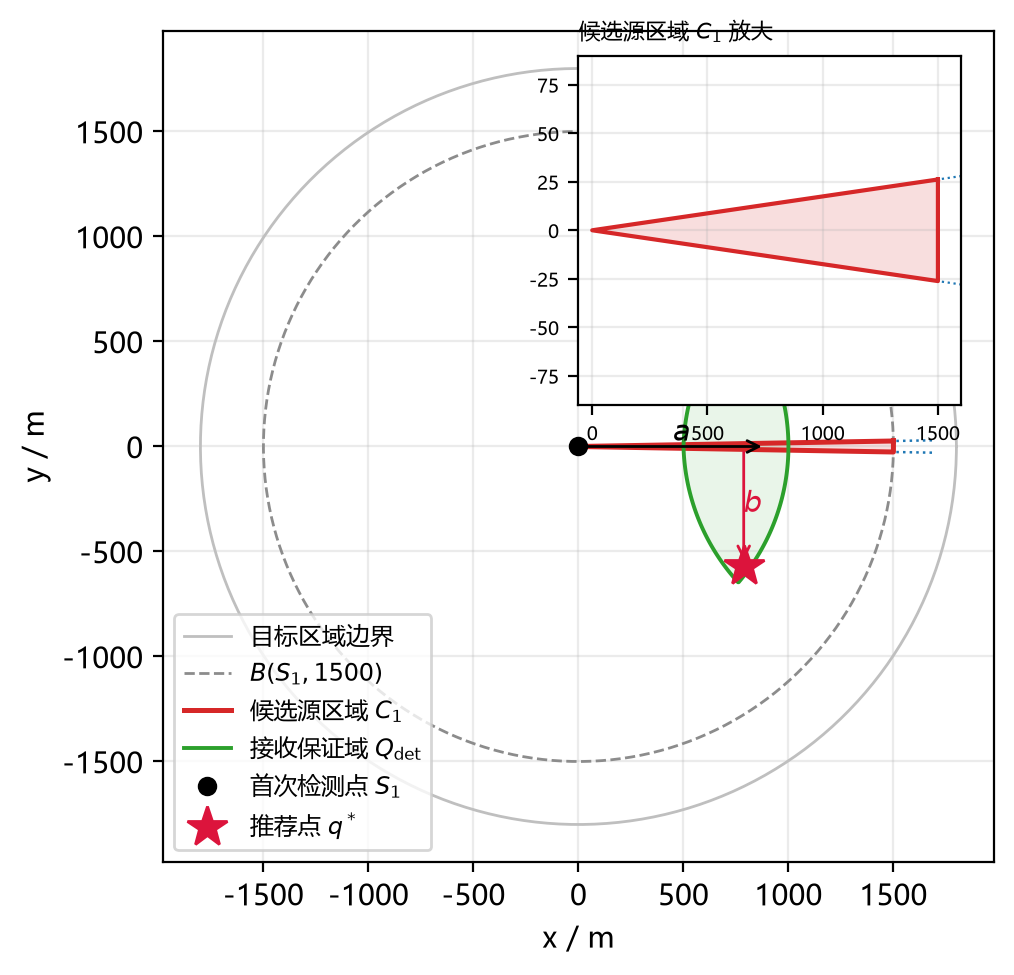
\includegraphics[width=\linewidth]{figures/q1q2_word/image3.png}
    \caption{候选区域与推荐点}
  \end{subfigure}\hfill
  \begin{subfigure}[t]{0.48\textwidth}
    \centering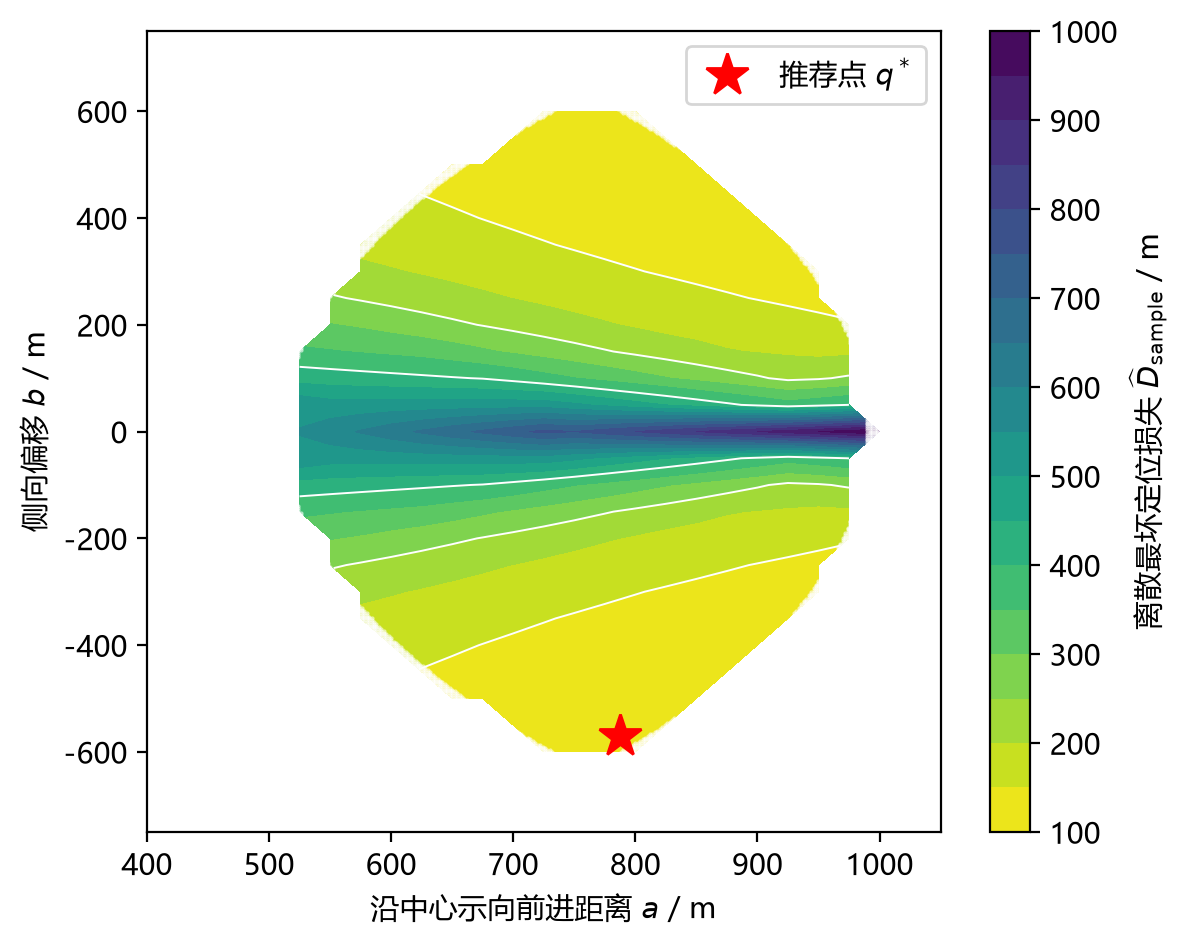
\includegraphics[width=\linewidth]{figures/q1q2_word/image4.png}
    \caption{离散最坏损失分布}
  \end{subfigure}

  \begin{subfigure}[t]{0.48\textwidth}
    \centering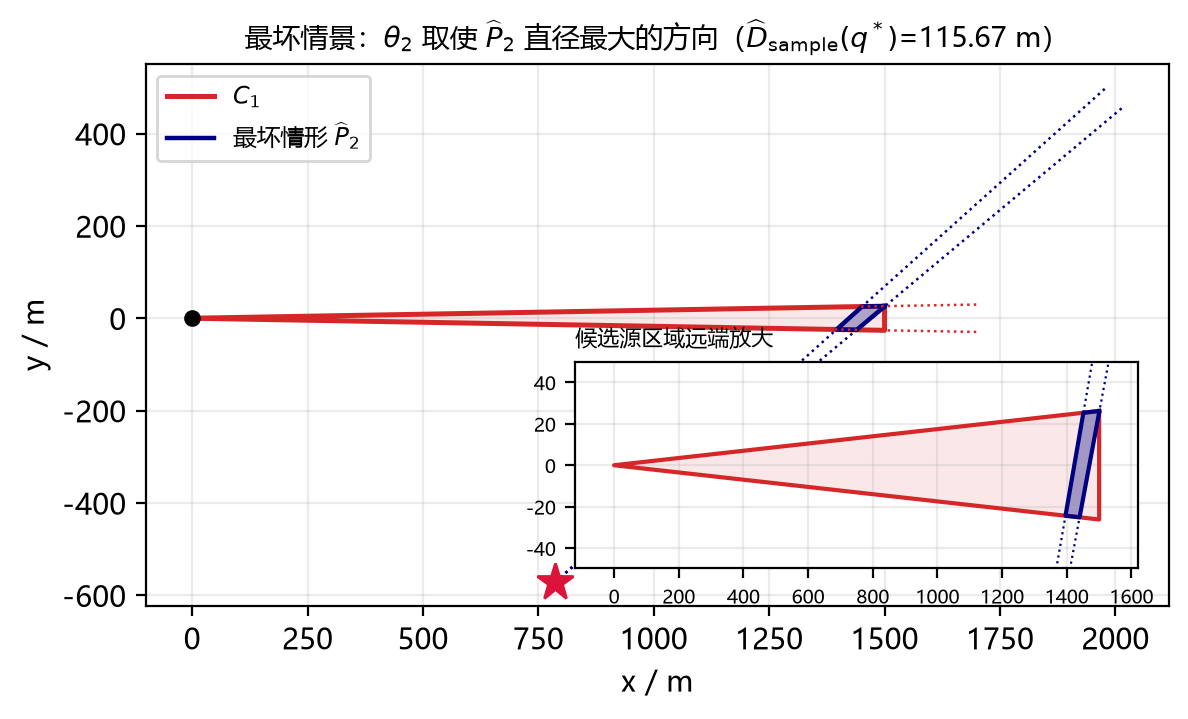
\includegraphics[width=\linewidth]{figures/q1q2_word/image5.png}
    \caption{推荐点处的最坏情形}
  \end{subfigure}\hfill
  \begin{subfigure}[t]{0.48\textwidth}
    \centering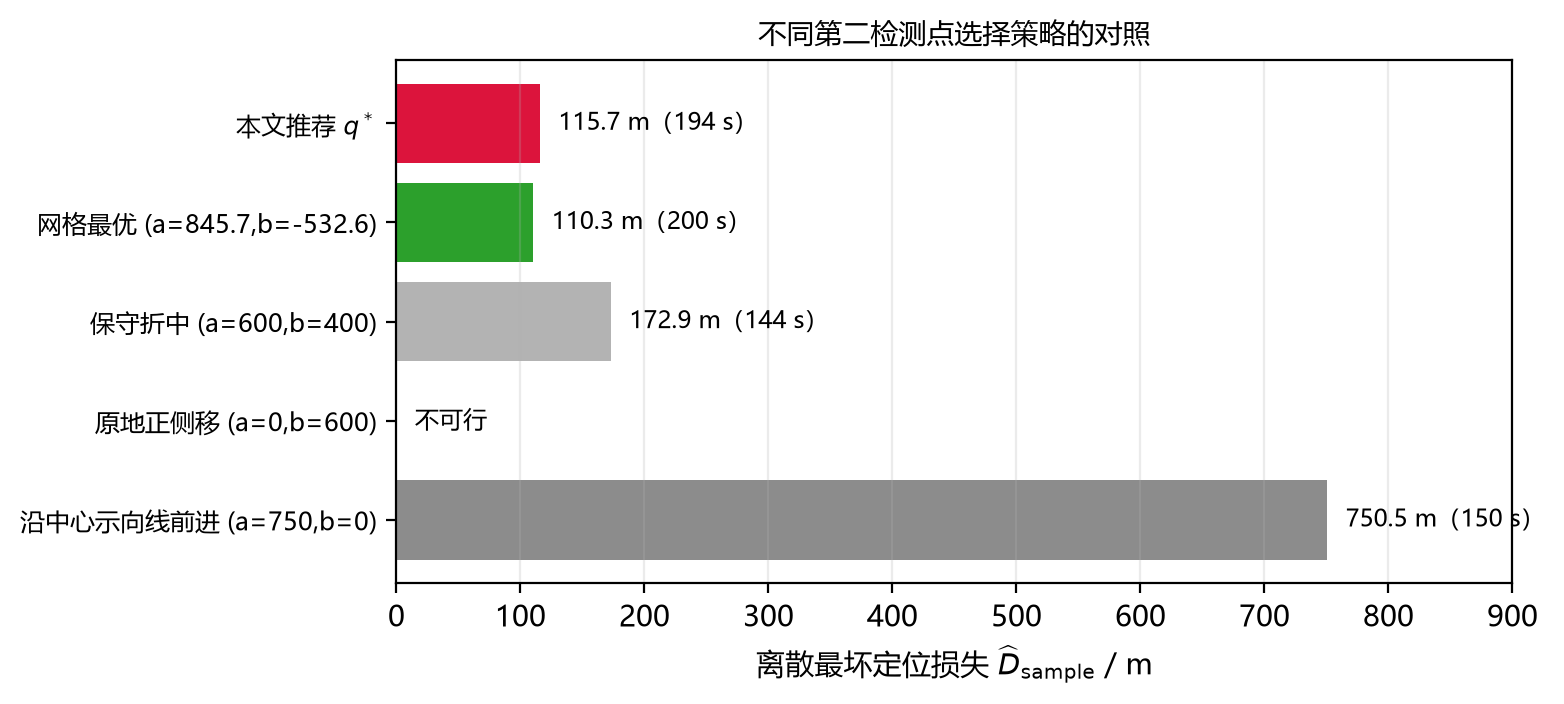
\includegraphics[width=\linewidth]{figures/q1q2_word/image6.png}
    \caption{不同第二检测点策略对照}
  \end{subfigure}
  \caption{问题二数值结果与几何检验}
  \label{fig:q2-results-panel}
\end{figure}

\subsection{数值检验方案}

为检查离散算法的可行性和数值稳定性，采用以下四类复核：
\begin{enumerate}
  \item \textbf{接收约束复核：}在候选点筛选阶段及最终推荐阶段，均计算检测点到 $\widehat C_{1,N}$ 全部顶点的最大距离，验证该值不超过 $1000$ 米并输出松弛量；
  \item \textbf{角度采样复核：}固定推荐点和外接多边形，分别采用 $L=61,121,241,481$，结果依次为 $112.35,115.67,115.67,115.67$ 米；
  \item \textbf{圆弧与网格复核：}固定推荐点和 $L=241$，圆弧外接边数与损失的对应关系为
  \[
    N=60,90,180,360
    \quad\Longrightarrow\quad
    115.67,115.67,115.67,115.62\ \text{米}.
  \]
  候选网格分段数为 $8,12,16$ 时，将各自最优点统一在 $N=180,L=241$ 下复核，结果分别为 $112.78,111.45,110.31$ 米；
  \item \textbf{基线策略对照：}在获得具体首次观测数据后，与沿中心示向线前进、原地垂直移动和随机选点三种策略比较样本评价值。
\end{enumerate}
角度与圆弧两类离散在该回归算例中已较稳定，而候选点网格仍呈改善趋势，因此只能说明当前层级的离散稳定性，不能据此证明连续全局最优。程序自检还覆盖角形平移、旋转卡壳与枚举对照、重复点线段直径、第二角形退化为线段、检测点位于候选多边形内部/边上/顶点/外部时的方位角覆盖，以及接收约束回代。

\subsection{策略结论}

综上，第二检测点在基于 $1000$ 米统一接收下界构造的保守可靠候选域 $Q_{\mathrm{cand}}$ 中选取。接收硬约束提供确定性保证；理论上以连续最坏定位损失为主要目标，以移动时间为次要目标。实际程序采用源区域外近似、扩大角域、有限角度采样和有限候选点网格得到离散代理值，并从相对近似最优集中选择移动时间较短的检测点。外近似与角域扩大具有保守方向，但有限采样没有未经证明的单侧误差保证，因此不把程序结果直接等同于连续最坏值或连续全局最优解。

本节的位置可行域更新和直径计算可作为后续在线定位的几何基础。对于全向源，可沿用基于距离下界的可靠检测点构造；在线更新时应保留全部历史观测约束，而不是只保留最近两次示向。对于定向源，还必须加入发射朝向条件或独立的保证搜索机制，不能仅凭距离约束保证接收。
